% Options for packages loaded elsewhere
\PassOptionsToPackage{unicode}{hyperref}
\PassOptionsToPackage{hyphens}{url}
\PassOptionsToPackage{dvipsnames,svgnames,x11names}{xcolor}
%
\documentclass[
  letterpaper,
  DIV=11,
  numbers=noendperiod,
  oneside]{scrartcl}

\usepackage{amsmath,amssymb}
\usepackage{iftex}
\ifPDFTeX
  \usepackage[T1]{fontenc}
  \usepackage[utf8]{inputenc}
  \usepackage{textcomp} % provide euro and other symbols
\else % if luatex or xetex
  \usepackage{unicode-math}
  \defaultfontfeatures{Scale=MatchLowercase}
  \defaultfontfeatures[\rmfamily]{Ligatures=TeX,Scale=1}
\fi
\usepackage{lmodern}
\ifPDFTeX\else  
    % xetex/luatex font selection
\fi
% Use upquote if available, for straight quotes in verbatim environments
\IfFileExists{upquote.sty}{\usepackage{upquote}}{}
\IfFileExists{microtype.sty}{% use microtype if available
  \usepackage[]{microtype}
  \UseMicrotypeSet[protrusion]{basicmath} % disable protrusion for tt fonts
}{}
\makeatletter
\@ifundefined{KOMAClassName}{% if non-KOMA class
  \IfFileExists{parskip.sty}{%
    \usepackage{parskip}
  }{% else
    \setlength{\parindent}{0pt}
    \setlength{\parskip}{6pt plus 2pt minus 1pt}}
}{% if KOMA class
  \KOMAoptions{parskip=half}}
\makeatother
\usepackage{xcolor}
\usepackage[left=1in,marginparwidth=2.0666666666667in,textwidth=4.1333333333333in,marginparsep=0.3in]{geometry}
\setlength{\emergencystretch}{3em} % prevent overfull lines
\setcounter{secnumdepth}{5}
% Make \paragraph and \subparagraph free-standing
\ifx\paragraph\undefined\else
  \let\oldparagraph\paragraph
  \renewcommand{\paragraph}[1]{\oldparagraph{#1}\mbox{}}
\fi
\ifx\subparagraph\undefined\else
  \let\oldsubparagraph\subparagraph
  \renewcommand{\subparagraph}[1]{\oldsubparagraph{#1}\mbox{}}
\fi


\providecommand{\tightlist}{%
  \setlength{\itemsep}{0pt}\setlength{\parskip}{0pt}}\usepackage{longtable,booktabs,array}
\usepackage{calc} % for calculating minipage widths
% Correct order of tables after \paragraph or \subparagraph
\usepackage{etoolbox}
\makeatletter
\patchcmd\longtable{\par}{\if@noskipsec\mbox{}\fi\par}{}{}
\makeatother
% Allow footnotes in longtable head/foot
\IfFileExists{footnotehyper.sty}{\usepackage{footnotehyper}}{\usepackage{footnote}}
\makesavenoteenv{longtable}
\usepackage{graphicx}
\makeatletter
\def\maxwidth{\ifdim\Gin@nat@width>\linewidth\linewidth\else\Gin@nat@width\fi}
\def\maxheight{\ifdim\Gin@nat@height>\textheight\textheight\else\Gin@nat@height\fi}
\makeatother
% Scale images if necessary, so that they will not overflow the page
% margins by default, and it is still possible to overwrite the defaults
% using explicit options in \includegraphics[width, height, ...]{}
\setkeys{Gin}{width=\maxwidth,height=\maxheight,keepaspectratio}
% Set default figure placement to htbp
\makeatletter
\def\fps@figure{htbp}
\makeatother
\newlength{\cslhangindent}
\setlength{\cslhangindent}{1.5em}
\newlength{\csllabelwidth}
\setlength{\csllabelwidth}{3em}
\newlength{\cslentryspacingunit} % times entry-spacing
\setlength{\cslentryspacingunit}{\parskip}
\newenvironment{CSLReferences}[2] % #1 hanging-ident, #2 entry spacing
 {% don't indent paragraphs
  \setlength{\parindent}{0pt}
  % turn on hanging indent if param 1 is 1
  \ifodd #1
  \let\oldpar\par
  \def\par{\hangindent=\cslhangindent\oldpar}
  \fi
  % set entry spacing
  \setlength{\parskip}{#2\cslentryspacingunit}
 }%
 {}
\usepackage{calc}
\newcommand{\CSLBlock}[1]{#1\hfill\break}
\newcommand{\CSLLeftMargin}[1]{\parbox[t]{\csllabelwidth}{#1}}
\newcommand{\CSLRightInline}[1]{\parbox[t]{\linewidth - \csllabelwidth}{#1}\break}
\newcommand{\CSLIndent}[1]{\hspace{\cslhangindent}#1}

\KOMAoption{captions}{tableheading}
\makeatletter
\makeatother
\makeatletter
\makeatother
\makeatletter
\@ifpackageloaded{caption}{}{\usepackage{caption}}
\AtBeginDocument{%
\ifdefined\contentsname
  \renewcommand*\contentsname{Table of contents}
\else
  \newcommand\contentsname{Table of contents}
\fi
\ifdefined\listfigurename
  \renewcommand*\listfigurename{List of Figures}
\else
  \newcommand\listfigurename{List of Figures}
\fi
\ifdefined\listtablename
  \renewcommand*\listtablename{List of Tables}
\else
  \newcommand\listtablename{List of Tables}
\fi
\ifdefined\figurename
  \renewcommand*\figurename{Figure}
\else
  \newcommand\figurename{Figure}
\fi
\ifdefined\tablename
  \renewcommand*\tablename{Table}
\else
  \newcommand\tablename{Table}
\fi
}
\@ifpackageloaded{float}{}{\usepackage{float}}
\floatstyle{ruled}
\@ifundefined{c@chapter}{\newfloat{codelisting}{h}{lop}}{\newfloat{codelisting}{h}{lop}[chapter]}
\floatname{codelisting}{Listing}
\newcommand*\listoflistings{\listof{codelisting}{List of Listings}}
\makeatother
\makeatletter
\@ifpackageloaded{caption}{}{\usepackage{caption}}
\@ifpackageloaded{subcaption}{}{\usepackage{subcaption}}
\makeatother
\makeatletter
\@ifpackageloaded{tcolorbox}{}{\usepackage[skins,breakable]{tcolorbox}}
\makeatother
\makeatletter
\@ifundefined{shadecolor}{\definecolor{shadecolor}{rgb}{.97, .97, .97}}
\makeatother
\makeatletter
\makeatother
\makeatletter
\@ifpackageloaded{sidenotes}{}{\usepackage{sidenotes}}
\@ifpackageloaded{marginnote}{}{\usepackage{marginnote}}
\makeatother
\makeatletter
\makeatother
\ifLuaTeX
  \usepackage{selnolig}  % disable illegal ligatures
\fi
\IfFileExists{bookmark.sty}{\usepackage{bookmark}}{\usepackage{hyperref}}
\IfFileExists{xurl.sty}{\usepackage{xurl}}{} % add URL line breaks if available
\urlstyle{same} % disable monospaced font for URLs
\hypersetup{
  pdftitle={Expert-guided Bayesian Optimisation for Human-in-the-loop Experimental Design of Known Systems},
  pdfauthor={Tom Savage; Antonio del Rio Chanona},
  pdfkeywords={Bayesian Optimisation, Expert
Guided, Human-In-The-Loop, Batch},
  colorlinks=true,
  linkcolor={blue},
  filecolor={Maroon},
  citecolor={Blue},
  urlcolor={Blue},
  pdfcreator={LaTeX via pandoc}}

\title{Expert-guided Bayesian Optimisation for Human-in-the-loop
Experimental Design of Known Systems}
\author{Tom Savage \and Antonio del Rio Chanona}
\date{2023-10-27}

\begin{document}
\maketitle
\ifdefined\Shaded\renewenvironment{Shaded}{\begin{tcolorbox}[enhanced, boxrule=0pt, interior hidden, borderline west={3pt}{0pt}{shadecolor}, sharp corners, frame hidden, breakable]}{\end{tcolorbox}}\fi

\renewcommand*\contentsname{Table of contents}
{
\hypersetup{linkcolor=}
\setcounter{tocdepth}{3}
\tableofcontents
}
\[
\DeclareMathOperator*{\argmax}{arg\,max}
\]

\hypertarget{abstract}{%
\subsection*{Abstract}\label{abstract}}
\addcontentsline{toc}{subsection}{Abstract}

Domain experts often possess valuable physical insights that are
overlooked in fully automated decision-making processes such as Bayesian
optimisation. In this article we apply high-throughput (batch) Bayesian
optimisation alongside anthropological decision theory to enable domain
experts to influence the selection of optimal experiments. Our
methodology exploits the hypothesis that humans are better at making
discrete choices than continuous ones and enables experts to influence
critical early decisions. At each iteration we solve an augmented
multi-objective optimisation problem across a number of alternate
solutions, maximising both the sum of their utility function values and
the determinant of their covariance matrix, equivalent to their total
variability. By taking the solution at the knee point of the Pareto
front, we return a set of alternate solutions at each iteration that
have both high utility values and are reasonably distinct, from which
the expert selects one for evaluation. We demonstrate that even in the
case of an uninformed practitioner, our algorithm recovers the regret of
standard Bayesian optimisation.

\hypertarget{introduction}{%
\subsection{Introduction}\label{introduction}}

Bayesian optimisation has been successfully applied in a number of
complex domains including engineering systems where derivatives are
often not available, such as those that involve simulation or propriety
software. By removing the human from decision-making processes in favour
of maximising statistical quantities such as expected improvement,
complex functions can be optimised in an efficient number of samples.
However, these engineering systems are often engaged with by domain
experts such as engineers or chemists, and as such the behaviour of the
underlying function cannot be considered completely unknown a-priori.
Therefore, there exists significant scope to take advantage of the
benefits of Bayesian optimisation in optimising expensive
derivative-free problems, whilst enabling domain experts to inform the
decision-making process, putting the human back into the loop. By
providing an optimal set of alternatives to an expert to select their
desired evaluation, we ensure that any one choice presents information
gain about the optimal solution. Simultaneously, we ensure the choices
are distinct enough to avoid the human making an effective gradient
calculation. Alternative solution information such as utility function
value, predictive output distribution and visualisations are provided to
the expert as a pseudo-likelihood. The decision-maker then effectively
performs discrete Bayesian reasoning, internally conditioning the
provided information with their own prior expertise and knowledge of the
solutions provided. In addition to improved convergence (depending on
the ability of the domain expert), our methodology enables improved
interpretability in higher dimensions, as the decision-maker has the
final say in what is evaluated. Our approach works with any utility
function and NSGA-II (Deb et al.
2002)\marginpar{\begin{footnotesize}\leavevmode\vadjust pre{\protect\hypertarget{ref-Deb2002}{}}%
Deb, K., A. Pratap, S. Agarwal, and T. Meyarivan. 2002. {``{A fast and
elitist multiobjective genetic algorithm: {NSGA}-{II}}.''} \emph{{IEEE}
Transactions on Evolutionary Computation} 6 (2): 182--97.
\url{https://doi.org/10.1109/4235.996017}.\vspace{2mm}\par\end{footnotesize}}
is applied for multi-objective optimisation, efficiently handling the
non-convex utility-space.\\
Figure~\ref{fig-overview} demonstrates our methodology

\begin{figure}

{\centering 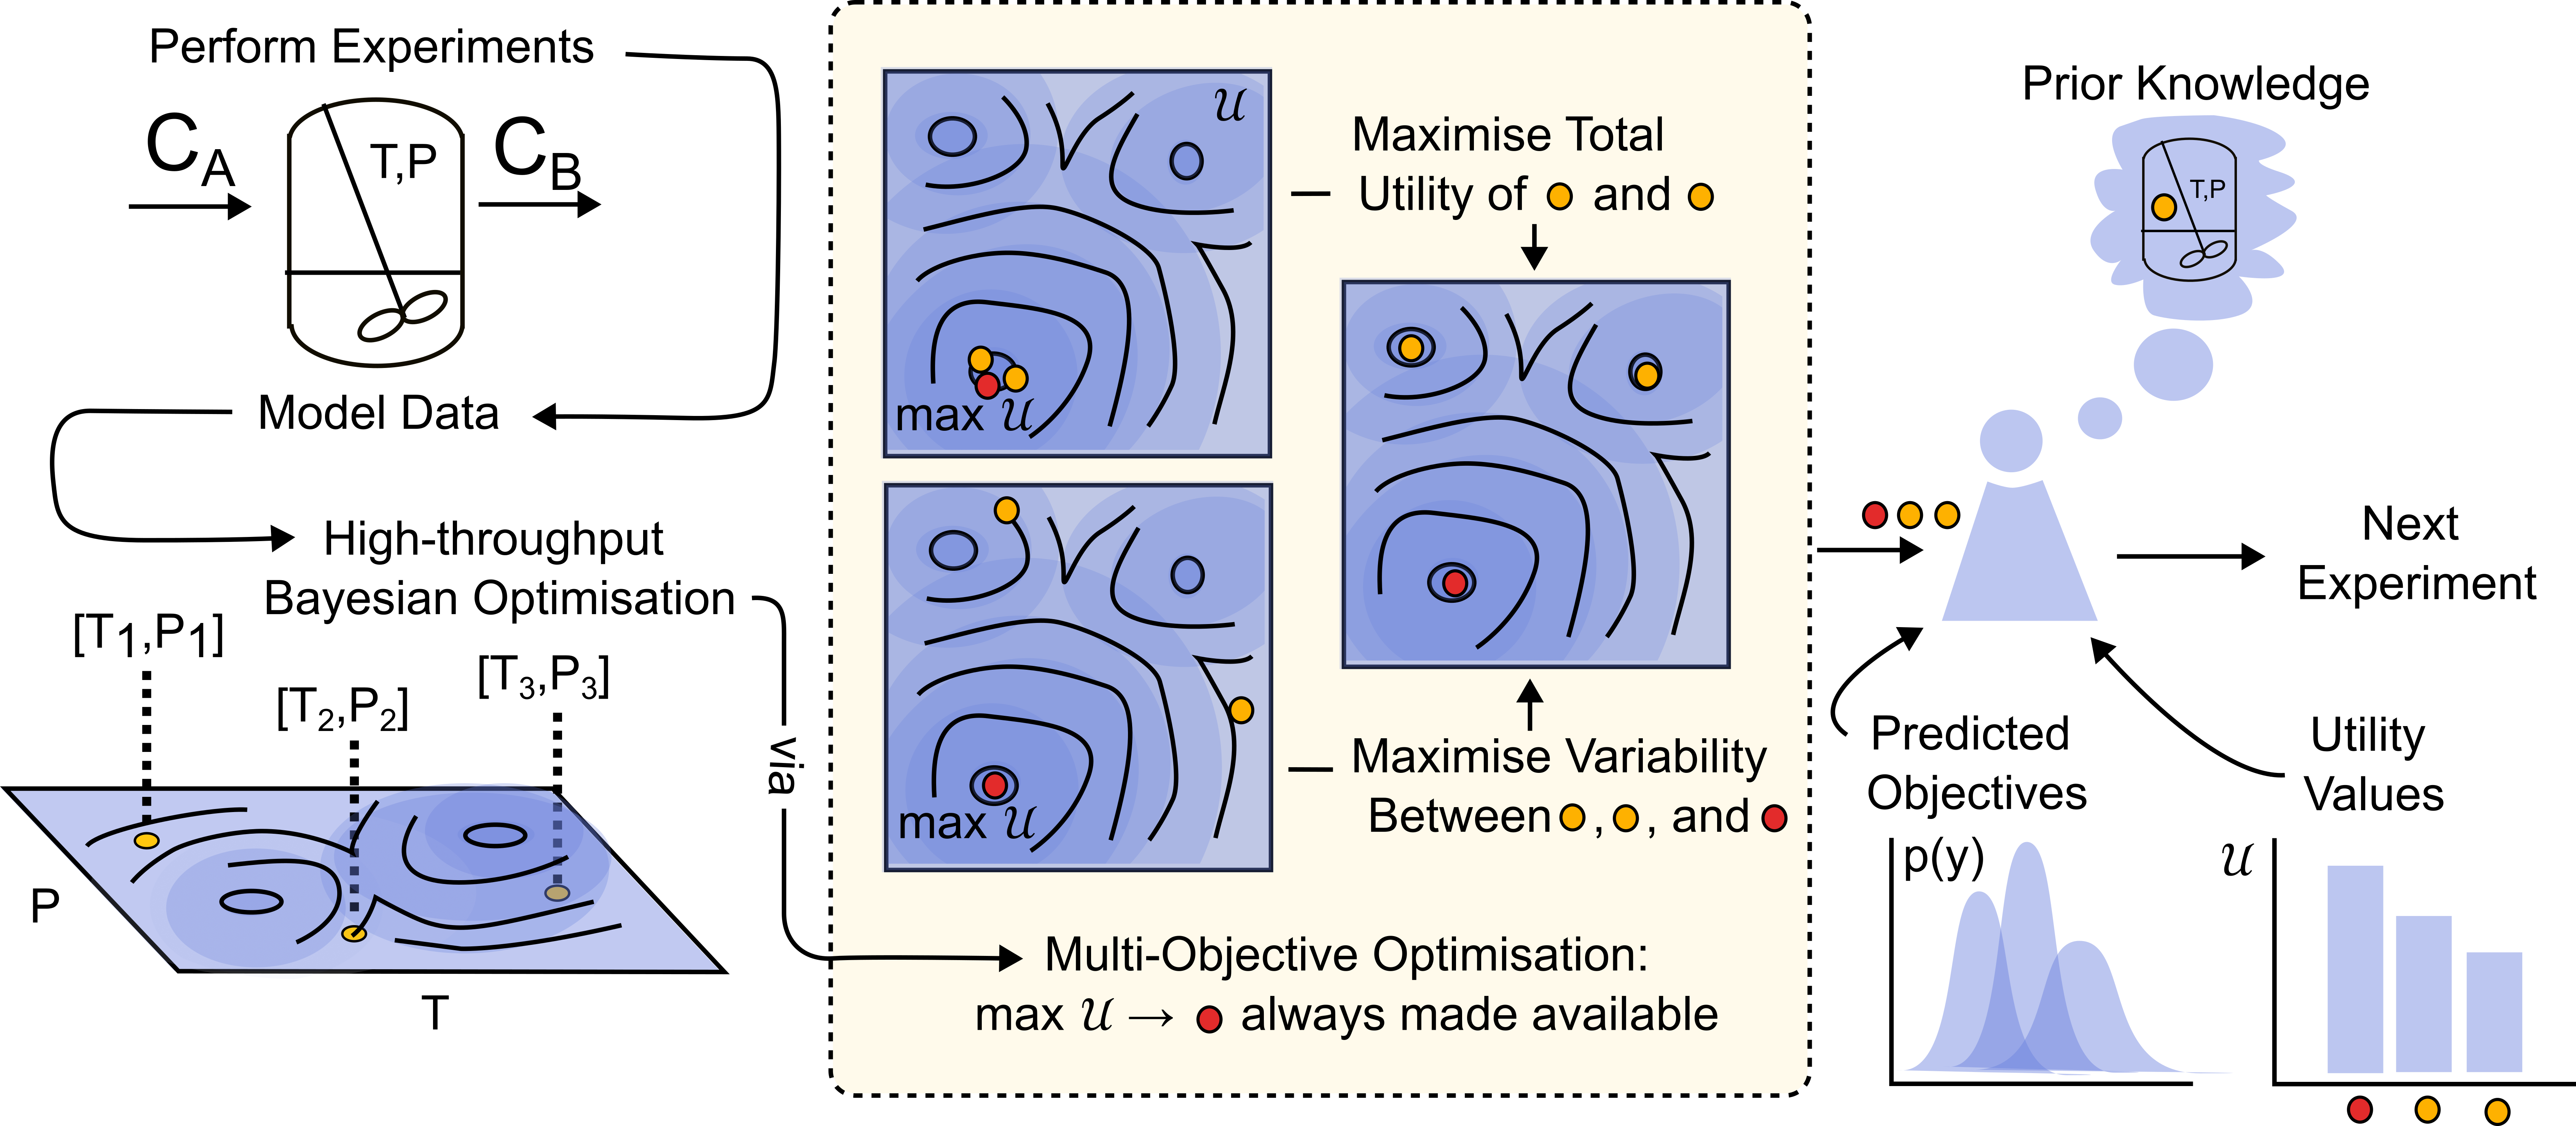
\includegraphics{overview_figure.png}

}

\caption{\label{fig-overview}Overview of our methodology, where an
augmented batch Bayesian optimisation problem is solved using
multi-objective optimisation, providing an expert with a set of
alternate solutions.}

\end{figure}

By allowing an expert to influence the experimental design through a
discrete decision step, we mitigate the expert needing to make
continuous decisions throughout, and do not rely on an expert `prior' of
the global optimum that necessarily must be defined before optimisation.
Approaches that rely on an expert-defined prior may need to redefine
this at significant human-cost throughout optimisation in light of new
information. Similarly, the expert has no influence over the actual
solutions evaluated and the optimisation is merely weighted towards
broad regions in solution-space.

\hypertarget{previous-work}{%
\subsection{Previous Work}\label{previous-work}}

(Kanarik et al.
2023)\marginpar{\begin{footnotesize}\leavevmode\vadjust pre{\protect\hypertarget{ref-Kanarik2023}{}}%
Kanarik, Keren J., Wojciech T. Osowiecki, Yu Lu, Dipongkar Talukder,
Niklas Roschewsky, Sae Na Park, Mattan Kamon, David M. Fried, and
Richard A. Gottscho. 2023. {``{Human-machine collaboration for improving
semiconductor process development}.''} \emph{Nature} 616 (7958):
707--11. \url{https://doi.org/10.1038/s41586-023-05773-7}.\vspace{2mm}\par\end{footnotesize}}
demonstrated that experts improve the initial convergence in Bayesian
optimisation for semiconductor processes. However, this can be
counterproductive in later stages. Algorithmic integration of expert
knowledge has been explored Hvarfner et al.
(2022)\marginpar{\begin{footnotesize}\leavevmode\vadjust pre{\protect\hypertarget{ref-Liu2022}{}}%
Liu, Peng. 2022. {``{Human-in-the-loop Bayesian Optimization with
No-Regret Guarantees},''} October.\vspace{2mm}\par\end{footnotesize}}.
(Hvarfner et al.
2022)\marginpar{\begin{footnotesize}\leavevmode\vadjust pre{\protect\hypertarget{ref-hvarfner2022pibo}{}}%
Hvarfner, Carl, Danny Stoll, Artur Souza, Marius Lindauer, Frank Hutter,
and Luigi Nardi. 2022. {``{\(\pi\)BO: Augmenting Acquisition Functions
with User Beliefs for Bayesian Optimization}.''}
\url{https://arxiv.org/abs/2204.11051}.\vspace{2mm}\par\end{footnotesize}}
and (Ramachandran et al.
2020)\marginpar{\begin{footnotesize}\leavevmode\vadjust pre{\protect\hypertarget{ref-Ramachandran2020}{}}%
Ramachandran, Anil, Sunil Gupta, Santu Rana, Cheng Li, and Svetha
Venkatesh. 2020. {``{Incorporating expert prior in Bayesian optimisation
via space warping}.''} \emph{Knowl. Based Syst.} 195 (May): 105663.
\url{https://doi.org/10.1016/j.knosys.2020.105663}.\vspace{2mm}\par\end{footnotesize}}
use user-defined priors to weight the acquisition function, while (Liu
2022)\marginpar{\begin{footnotesize}\leavevmode\vadjust pre{\protect\hypertarget{ref-Liu2022}{}}%
Liu, Peng. 2022. {``{Human-in-the-loop Bayesian Optimization with
No-Regret Guarantees},''} October.\vspace{2mm}\par\end{footnotesize}}
diminishes this weight over time. These methods are static and don't
allow real-time expert input. (Gupta et al.
2023)\marginpar{\begin{footnotesize}\leavevmode\vadjust pre{\protect\hypertarget{ref-BOMuse}{}}%
Gupta, Sunil, Alistair Shilton, Arun Kumar A, Shannon Ryan, Majid
Abdolshah, Hung Le, Santu Rana, Julian Berk, Mahad Rashid, and Svetha
Venkatesh. 2023. {``{BO-Muse: A human expert and AI teaming framework
for accelerated experimental design}.''}
\url{https://doi.org/10.48550/ARXIV.2303.01684}.\vspace{2mm}\par\end{footnotesize}}
allows continuous expert involvement, using a linear Gaussian process to
approximate human intuition, achieving sub-linear regret bounds. (Kumar
et al.
2022)\marginpar{\begin{footnotesize}\leavevmode\vadjust pre{\protect\hypertarget{ref-av2022human}{}}%
Kumar, A V, Arun, Santu Rana, Alistair Shilton, and Svetha Venkatesh.
2022. {``{Human-AI Collaborative Bayesian Optimisation}.''}
\emph{Advances in Neural Information Processing Systems} 35: 16233--45.\vspace{2mm}\par\end{footnotesize}}
and (Maus et al.
2022)\marginpar{\begin{footnotesize}\leavevmode\vadjust pre{\protect\hypertarget{ref-robot}{}}%
Maus, Natalie, Kaiwen Wu, David Eriksson, and Jacob Gardner. 2022.
{``{Discovering Many Diverse Solutions with Bayesian Optimization}.''}
\url{https://doi.org/10.48550/ARXIV.2210.10953}.\vspace{2mm}\par\end{footnotesize}}
present similar frameworks, offering alternative solutions for
evaluation, with the expert making the final decision latterly in a
molecular design setting.

\hypertarget{method}{%
\subsection{Method}\label{method}}

We first maximise a given utility function \(\mathcal{U}\) for a given
dataset \(\mathcal{D}_t:= \{(\mathbf{x}_i,y_i)\}_{i=1}^t\):

\begin{equation}\protect\hypertarget{eq-standard-bo}{}{
   \mathbf{x}^* = \argmax_{x\in\mathcal{X}\subseteq\mathbb{R}^n} \; \mathcal{U}(x),
}\label{eq-standard-bo}\end{equation}

resulting in the optimal next evaluation, \(\mathbf{x}^*\), in a utility
sense. Let \(p\) be the number of alternate solutions provided to the
expert and construct the decision variable matrix
\(\mathbf{X} \in \mathbb{R}^{(p-1)\times n}\) by concatenating \(p-1\)
alternate solutions
\(\mathbf{X} := [\mathbf{x}_1,\dots,\mathbf{x}_{p-1}]\). We then define
the high-throughput (batch) utility function \(\hat{\mathcal{U}}\) which
is specified as the sum of the individual utilities of alternate
solutions within \(\mathbf{X}\)

\begin{align}
    \hat{\mathcal{U}}(\mathbf{X}) = \sum_{i=0}^{p-1} \mathcal{U}(\mathbf{X}_i).
\end{align} Similarly, we introduce \(\hat{\mathcal{S}}\) as a measure
for capturing the variability among both the optimal and alternative
solutions. Specifically, let \(\hat{\mathcal{S}}\) be the determinant of
the covariance matrix \(K_{\mathbf{X}_{\text{aug}}}\) for the augmented
set \(\mathbf{X}_{\text{aug}}= \mathbf{X} \cup \mathbf{x}^*\):
\begin{align*}
 \hat{\mathcal{S}}(\mathbf{X},\mathbf{x}^*) &= |K_{\mathbf{X_{\text{aug}}}}| \\
 K_{\mathbf{X}_{\text{aug}}} &= [k(\mathbf{X}_{\text{aug},i},\mathbf{X}_{\text{aug},j})]^p_{i,j=1}
\end{align*} \(\hat{\mathcal{S}}\) quantifies the `volume of
information' spanned by the alternative solutions \(\mathbf{X}\) as well
as the optimal solution \(\mathbf{x}^*\). Maximising
\(\hat{\mathcal{U}}\) will result in all alternative solutions proposed
being the same as \(\mathbf{x}^*\), that is
\([\mathbf{x}^*_1,\dots,\mathbf{x}^*_{p-1}]\). Contrary to this,
maximising \(\hat{\mathcal{S}}\) will result in a set of solutions that
are maximally-spaced both with respect to other alternatives, but also
\(\mathbf{x}^*\). At iteration \(t\), we then solve the following
multi-objective optimisation problem:
\begin{align}\label{multi-objective}
    [\mathbf{X}^*_1,\dots,\mathbf{X}^*_m] = \max_{\mathbf{X}} \; \left(\hat{\mathcal{U}}(\mathbf{X};\mathcal{D}_t),\hat{\mathcal{S}}(\mathbf{X},\mathbf{x}^*)\right),
\end{align} resulting in a set of \(m\) solutions along the Pareto front
of both objectives. From this we define \(\mathbf{X}^*_{k}\) as the
solution at knee-point of the Pareto front. The \(p-1\) solutions
contained within \(\mathbf{X}^*_k\) optimally trade off the sum of their
utility values, with their variability. This ensures that when provided
to an expert, alongside \(\mathbf{x}^*\), any individual solution will
have high expected information gain, and the solutions themselves will
be distinct enough to ensure the expert isn't made to make an effective
gradient calculation.\\
The practitioner is then made to choose a solution to evaluate from this
set of alternatives. To do so, they are provided with information such
as the utility value of each solution, expected output distributions
(obtained from the Gaussian process), and information regarding previous
solutions that they may wish to draw upon. In doing so, the practitioner
effectively performs an internal discrete Bayesian reasoning,
conditioning previous prior information and expert opinion with the
mathematical quantities provided to make an informed decision. Our
algorithm can be located within the Appendix.

Figure~\ref{fig-behav} demonstrates the intended behaviour of our
approach. We present a one-dimensional case study, optimising a function
obtained through sampling a Gaussian process prior, specified by a
Matern 5/2 kernel with lengthscale \(l=0.5\). In this case study we
provide 3 alternatives to an expert, who's choice we select randomly. We
provide details of optimisation methods and hyper-parameters within the
Appendix.

\begin{figure}

\begin{minipage}[t]{\linewidth}

{\centering 

\raisebox{-\height}{

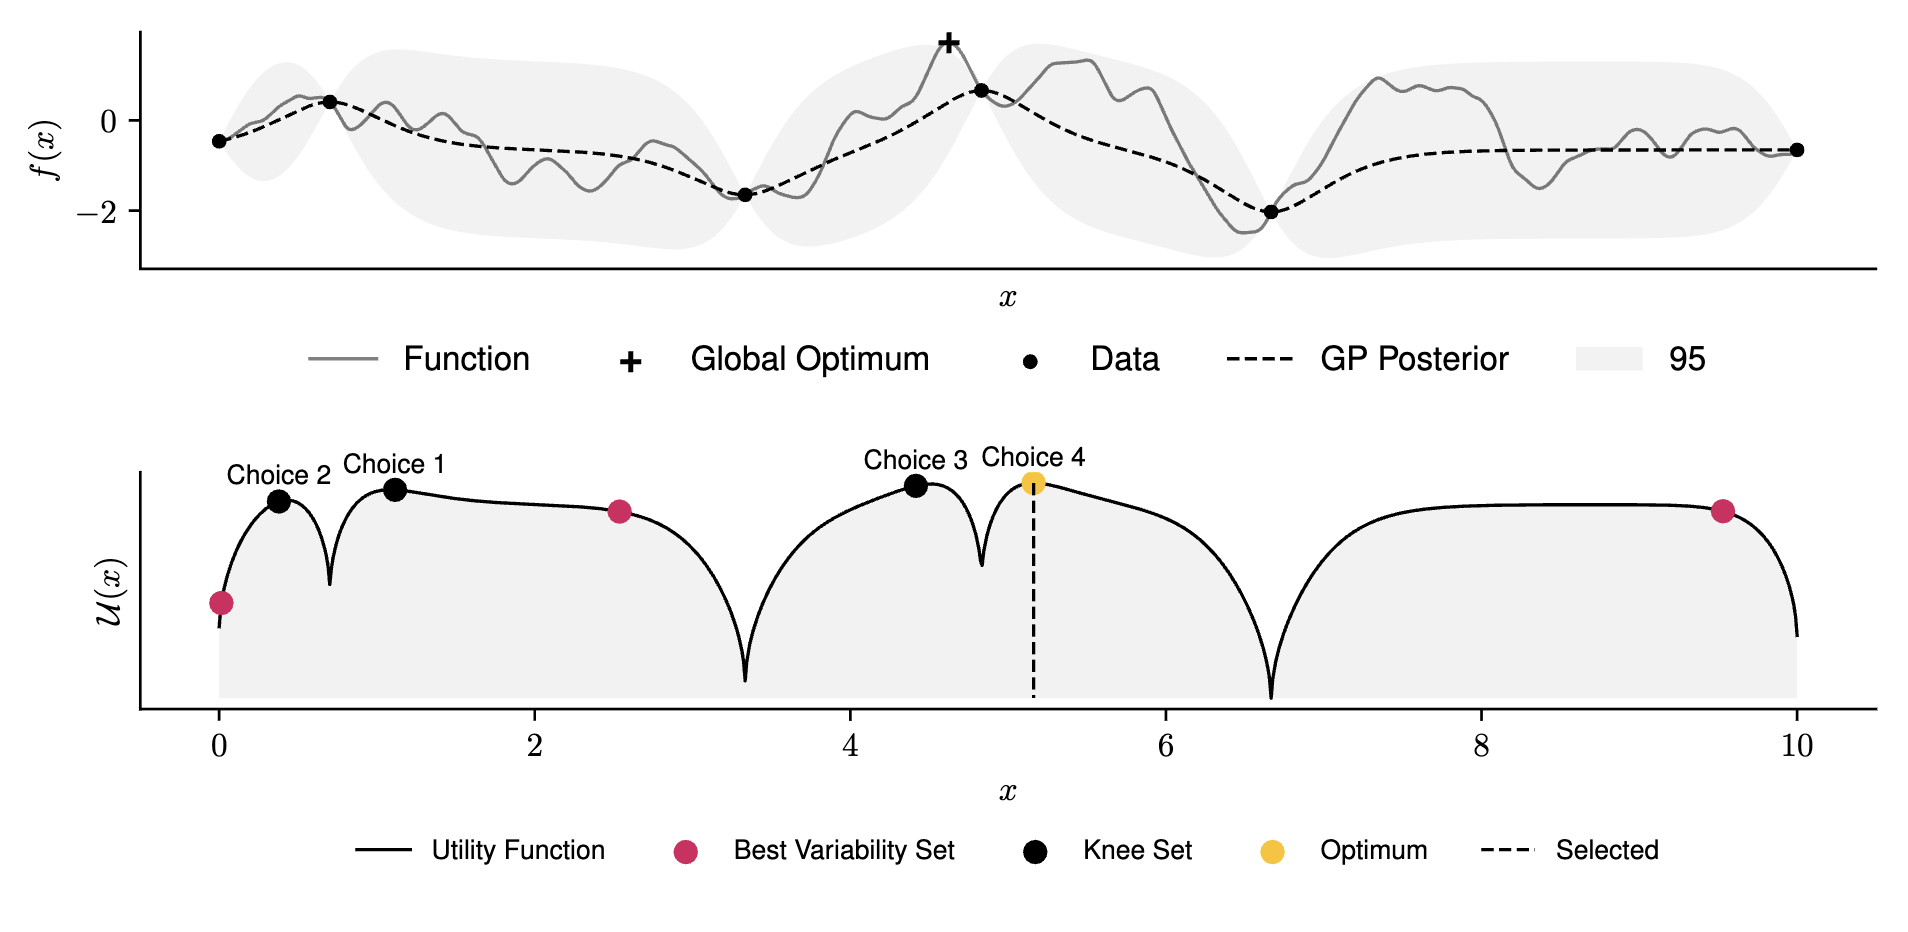
\includegraphics{utility.png}

}

}

\subcaption{\label{fig-util}The objective function and utility function
after 6 function evaluations. The 3 alternative solutions that maximise
the solution distance can be seen in red, whilst the black solutions
denote those contained within the knee-solution of the high-throughput
multi-objective problem. The yellow optimal solution is included
alongside these two alternatives to an expert. In this case choice 4 is
selected randomly from the 3 alternatives and the optimum.}
\end{minipage}%
\newline
\begin{minipage}[t]{\linewidth}

{\centering 

\raisebox{-\height}{

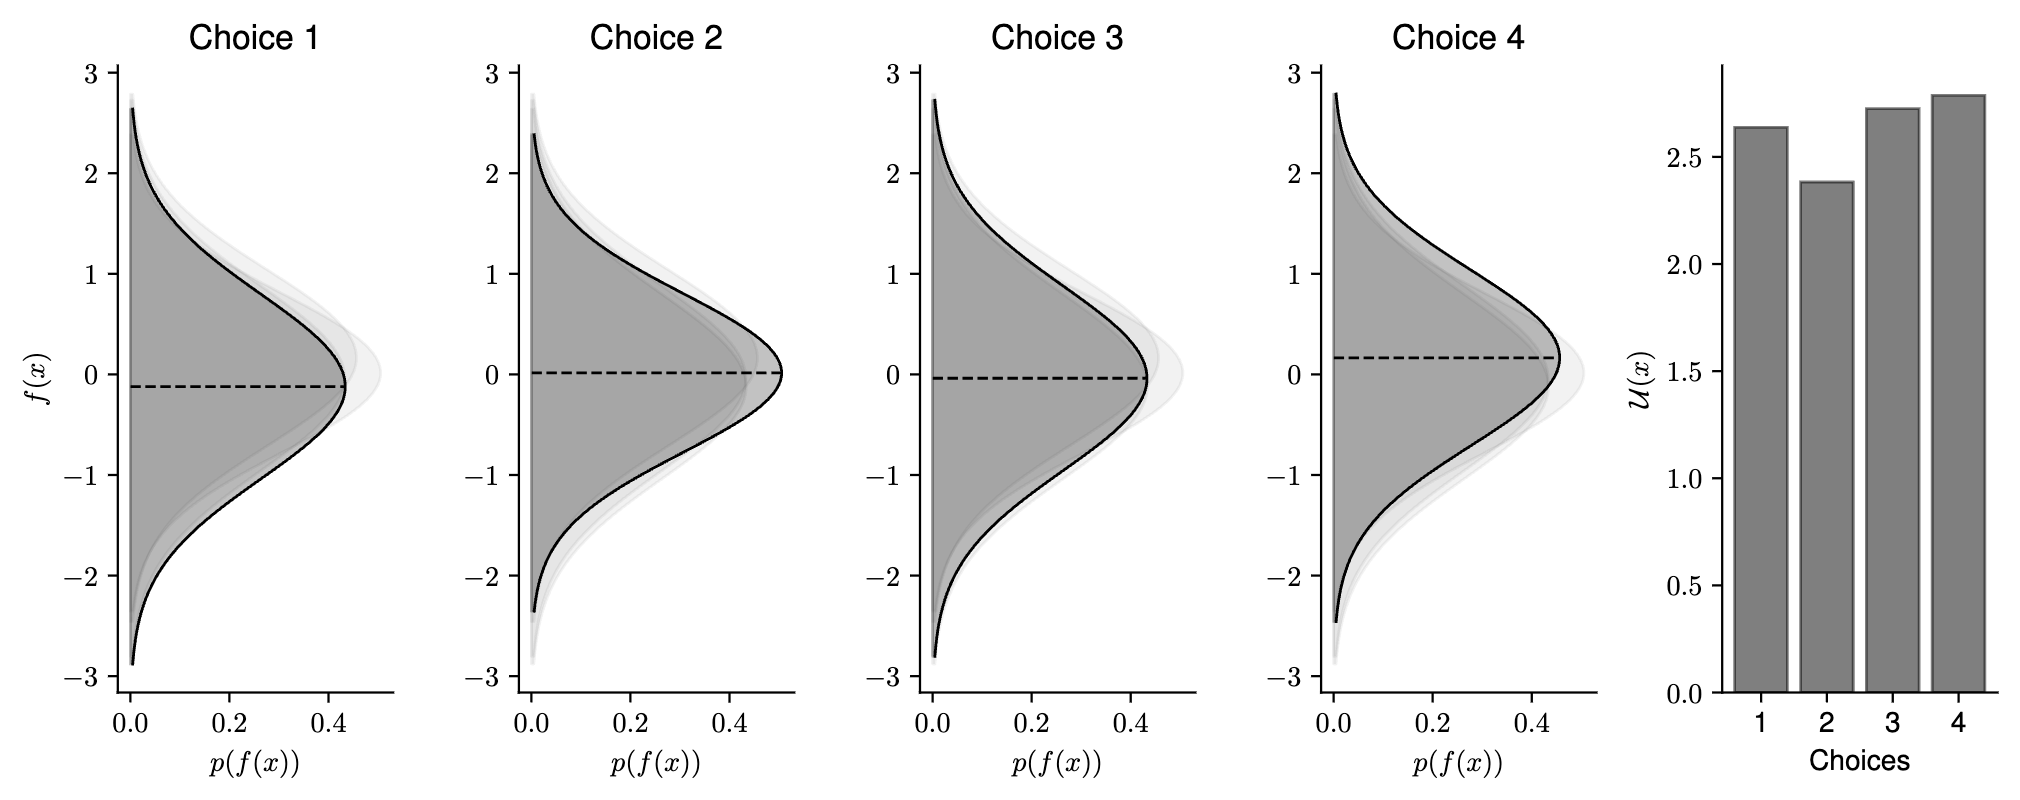
\includegraphics{choices.png}

}

}

\subcaption{\label{fig-choices}The information provided to the expert
regarding the three alternative solutions. In this case choice 1 and
choice 3 have relatively similar utility values and predicted output
distributions to choice 4 (the optimal of the acquisition function). The
expert is then allowed to distinguish between these similar solutions in
a way the computer cannot through their prior domain knowledge. By
conditioning their prior information on the given values, the expert is
effectively performing internal Bayesian reasoning.}
\end{minipage}%

\caption{\label{fig-behav}A standard iteration of our approach on a
one-dimensional case-study.}

\end{figure}

\hypertarget{computational-results-discussion}{%
\subsection{Computational Results \&
Discussion}\label{computational-results-discussion}}

To assess our approach, we benchmark it against standard Bayesian
optimisation. In order to incorporate and assess human interaction in an
automated manner, we hypothesise a number of different human behaviours.
The `Expert' practitioner represents an ideal, where the best solution
(that is the one with the highest true objective value) is always
selected. Equivalently, to test the performance of our approach under
the influence of a practitioner with misaligned knowledge, we present an
`Adversarial' practitioner who consistently selects the solution with
the lowest true objective value. In addition, we present a probabilistic
practitioner, who selects the solution with the best true objective
value with some probability. Finally, we present the behaviour of a
`Trusting' practitioner who selects the solution with the largest
utility (as these values are presented), equivalent to standard Bayesian
optimisation as this solution is obtained through standard single
objective optimisation (Equation~\ref{eq-standard-bo}). In practice, the
expert will condition the information provided with their prior beliefs.
In our approach this includes information regarding the expected
distribution of the objective of each solution, as well as the utility
value of each solution. Whilst we cannot benchmark real human behaviour
due to the random nature of the objective functions, and practical
issues, the behaviours described summarise key aspects in order to
generate useful insights into our approach, we leave this for future
work. The human behaviours applied are summarised within
Table~\ref{tbl-behav}.

\hypertarget{tbl-behav}{}
\begin{longtable}[]{@{}
  >{\raggedright\arraybackslash}p{(\columnwidth - 2\tabcolsep) * \real{0.5000}}
  >{\raggedright\arraybackslash}p{(\columnwidth - 2\tabcolsep) * \real{0.5000}}@{}}
\caption{\label{tbl-behav}Human Behaviours Applied for
Benchmarking}\tabularnewline
\toprule\noalign{}
\begin{minipage}[b]{\linewidth}\raggedright
\textbf{Behaviour Type}
\end{minipage} & \begin{minipage}[b]{\linewidth}\raggedright
\textbf{Description}
\end{minipage} \\
\midrule\noalign{}
\endfirsthead
\toprule\noalign{}
\begin{minipage}[b]{\linewidth}\raggedright
\textbf{Behaviour Type}
\end{minipage} & \begin{minipage}[b]{\linewidth}\raggedright
\textbf{Description}
\end{minipage} \\
\midrule\noalign{}
\endhead
\bottomrule\noalign{}
\endlastfoot
Expert & Selects the solution with the best true function value. \\
Adversarial & Selects the solution with the worst true function
value. \\
Trusting & Selects the solution with the maximum utility value. \\
p(Best) & Selects the solution with the best true function value with
probability p(Best), otherwise selects a random solution. \\
\end{longtable}

We perform optimisation over 50 functions, each representing a sample
from a Gaussian process prior with lengthscale 0.3 using the
upper-confidence bound (UCB) utility function. Figure~\ref{fig-res}
demonstrates the average and standard deviation of simple regret, and
average regret (both defined within Garnett
(2023)\marginpar{\begin{footnotesize}\leavevmode\vadjust pre{\protect\hypertarget{ref-Garnett2023}{}}%
Garnett, Roman. 2023. \emph{{Bayesian Optimization}}. Cambridge
University Press. \url{https://doi.org/10.1017/9781108348973}.\vspace{2mm}\par\end{footnotesize}})
for each human behaviour across 1D and 2D objective functions.\\
Results for 5D, and specific functions can be located within the
Appendix.

\begin{figure}

\begin{minipage}[t]{\linewidth}

{\centering 

\raisebox{-\height}{

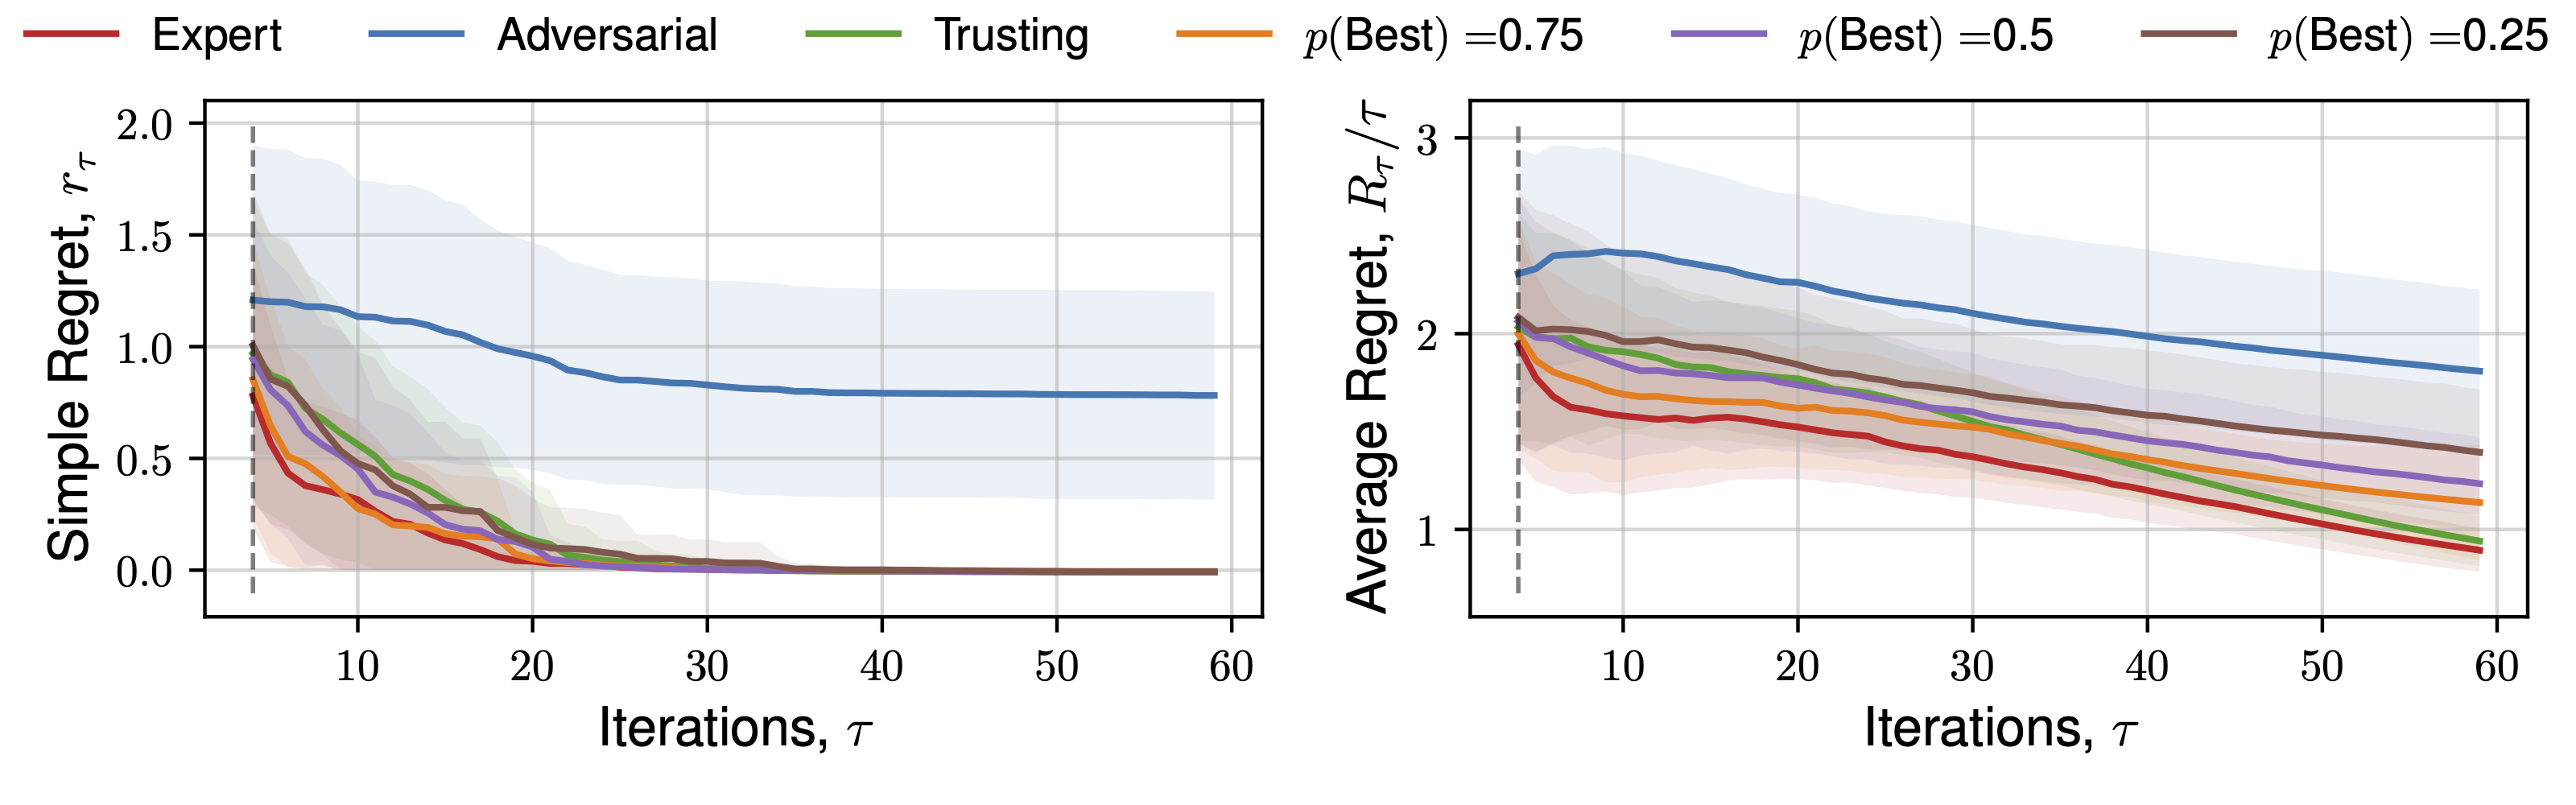
\includegraphics{overall_regret_aq_UCB_d_1.png}

}

}

\subcaption{\label{fig-1D}Average regret quantities over 1D objective
functions.}
\end{minipage}%
\newline
\begin{minipage}[t]{\linewidth}

{\centering 

\raisebox{-\height}{

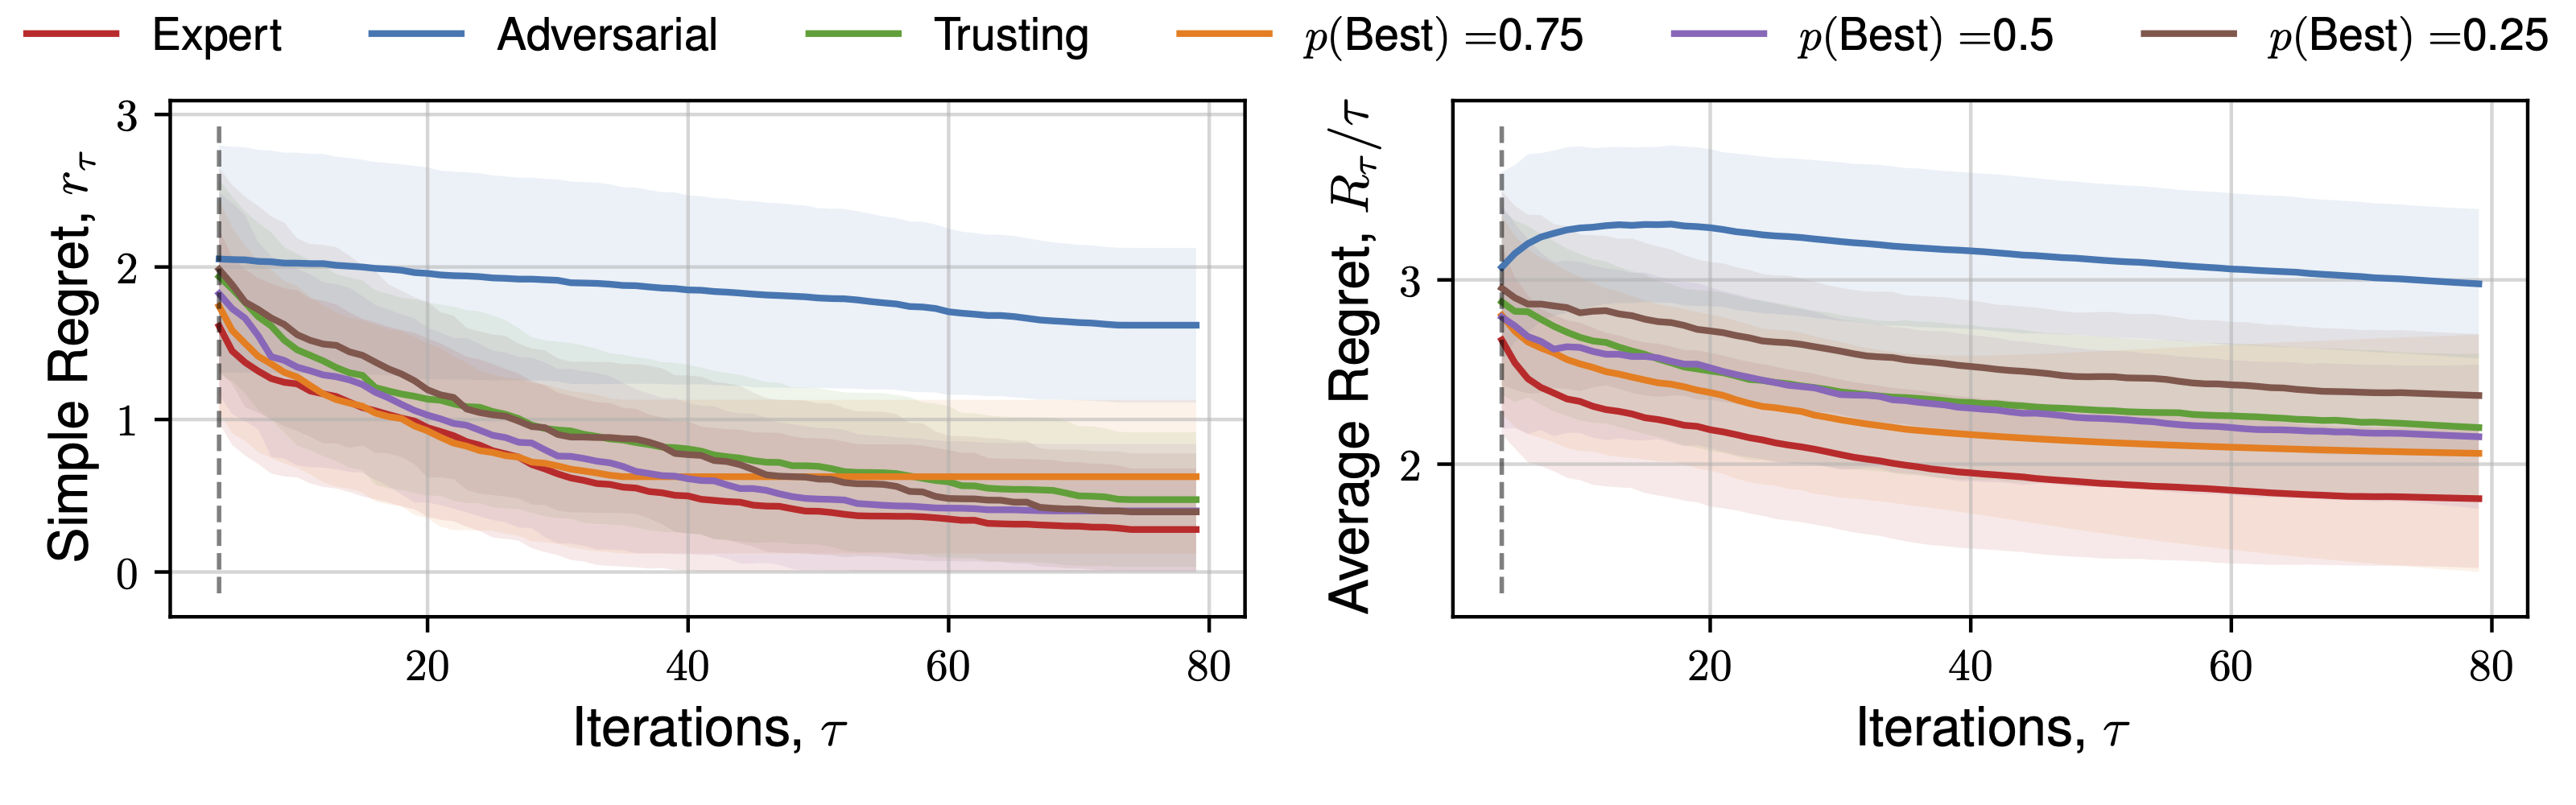
\includegraphics{overall_regret_aq_UCB_d_2.png}

}

}

\subcaption{\label{fig-2D}Average regret quantities over 2D objective
functions.}
\end{minipage}%

\caption{\label{fig-res}Regret expectation over 50 functions,
\(f \sim \mathcal{GP}(\mu \equiv 0, K_M (d,\nu = 0.3))\) where \(K_M\)
is the Mat\textquotesingle ern 5/2 kernel function. 4 alternate choices
are presented to the practitioner, and the utility function
\(\mathcal{U}(x)\) used is the upper-confidence bound.}

\end{figure}

The expectation of average regret tends towards zero for all behaviours,
indicating empirical convergence. Focusing on results from the set of 1D
functions, an `Expert' provides improved convergence than standard
Bayesian optimisation (`Trusting') throughout all iterations, with
benefits diminishing throughout the later stages, where the standard
automated approach recovers the `Expert' average regret value,
confirming previous observations regarding the importance of human input
throughout earlier iterations, and conversely diminishing importance of
expert opinion during `fine-tuning' Kanarik et al.
(2023)\marginpar{\begin{footnotesize}\leavevmode\vadjust pre{\protect\hypertarget{ref-Kanarik2023}{}}%
Kanarik, Keren J., Wojciech T. Osowiecki, Yu Lu, Dipongkar Talukder,
Niklas Roschewsky, Sae Na Park, Mattan Kamon, David M. Fried, and
Richard A. Gottscho. 2023. {``{Human-machine collaboration for improving
semiconductor process development}.''} \emph{Nature} 616 (7958):
707--11. \url{https://doi.org/10.1038/s41586-023-05773-7}.\vspace{2mm}\par\end{footnotesize}}.
Improved convergence of simple regret occurs in cases where the
practitioner selects the `best' solution from a set 75\%, 50\%, and to a
lesser extent 25\% of the time out of 4 available choices, similarly
reflected in trends across average regret. The results demonstrated in
Figure~\ref{fig-res} indicate the potential for our approach to improve
the convergence of Bayesian optimisation even in cases where the
practitioner is correct about a decision only partially. When the expert
makes a random selection (\(p(\text{Best}) = 0.25\), for 4 alternate
solutions), standard Bayesian optimisation convergence is recovered,
indicating the effectiveness of the choices presented by asking a
practitioner to select between distinct solutions, each of which
individually has a high utility value. This is reflected throughout 1D,
2D and 5D functions. Only in the case where the practitioner actively
selects the worst solution (i.e.~they are misaligned), is performance
worse. In higher-dimensions an adversarial practitioner performs worse,
as they are performing inefficient space-filling in an increasingly
larger volume before good solutions are found.

The methodology we present may also be interpreted as an approach for
high-throughput/batch Bayesian optimisation, with an additional
preference for solutions that are well-distributed throughout the search
space. Our intention for future work is to benchmark it against other
existing batch Bayesian optimisation methodologies González et al.
(2015)\marginpar{\begin{footnotesize}\leavevmode\vadjust pre{\protect\hypertarget{ref-local_pen}{}}%
González, Javier, Zhenwen Dai, Philipp Hennig, and Neil D. Lawrence.
2015. {``{Batch Bayesian Optimization via Local Penalization}.''}
\url{https://doi.org/10.48550/ARXIV.1505.08052}.\vspace{2mm}\par\end{footnotesize}},
including those with similar multi-objective formulations (Bischl et al.
(2014)\marginpar{\begin{footnotesize}\leavevmode\vadjust pre{\protect\hypertarget{ref-Bischl2014}{}}%
Bischl, Bernd, Simon Wessing, Nadja Bauer, Klaus Friedrichs, and Claus
Weihs. 2014. {``{{MOI}-{MBO}: Multiobjective Infill for Parallel
Model-Based Optimization}.''} In \emph{Lecture Notes in Computer
Science}, 173--86. Springer International Publishing.
\url{https://doi.org/10.1007/978-3-319-09584-4_17}.\vspace{2mm}\par\end{footnotesize}},Habib,
Singh, and Ray
(2016)\marginpar{\begin{footnotesize}\leavevmode\vadjust pre{\protect\hypertarget{ref-Habib2016}{}}%
Habib, Ahsanul, Hemant Kumar Singh, and Tapabrata Ray. 2016. {``{A
multi-objective batch infill strategy for efficient global
optimization}.''} In \emph{2016 {IEEE} Congress on Evolutionary
Computation ({CEC})}. {IEEE}.
\url{https://doi.org/10.1109/cec.2016.7744341}.\vspace{2mm}\par\end{footnotesize}},Maus
et al.
(2022)\marginpar{\begin{footnotesize}\leavevmode\vadjust pre{\protect\hypertarget{ref-robot}{}}%
Maus, Natalie, Kaiwen Wu, David Eriksson, and Jacob Gardner. 2022.
{``{Discovering Many Diverse Solutions with Bayesian Optimization}.''}
\url{https://doi.org/10.48550/ARXIV.2210.10953}.\vspace{2mm}\par\end{footnotesize}}).
We will also investigate to what extent large-language models can
perform the selection step.

\hypertarget{appendix}{%
\subsection*{Appendix}\label{appendix}}
\addcontentsline{toc}{subsection}{Appendix}

\hypertarget{algorithm}{%
\subsubsection*{Algorithm}\label{algorithm}}
\addcontentsline{toc}{subsubsection}{Algorithm}




\end{document}
